\documentclass[11pt,a4paper]{article}

\usepackage{amsmath} %for mathemathic formulas
\usepackage{amssymb}
\usepackage[ngerman]{babel} %for the german language by the spellling reform (without the package the date would look like April 20, 2020)
\usepackage{enumitem} %for enumeration surrounding 
\usepackage{graphicx} %for pictures
\usepackage{siunitx}
\usepackage{float}

\title{Blatt 12}
\date{\today}
\author{Hannah Rotgeri \and Feline Heinzelmann}

\begin{document}
    \maketitle


	\begin{itemize}
		\item[a)] 
			Teilchen in einem Synchrotron bewegen sich auf einer Kreisbahn
			und erfahren demnach eine Beschleunigung.
			Da beschleunigte Ladungen Photonen emittieren,
			wird Synchrotronstrahlung abgestrahlt.

		\item[b)]
			Das kontinuerliche Spektrum hat ein Maximum bei kleinen Frequenzen und 
			wird durch die kritische Energie in zwei gleichgroße Leistungsintegrale geteilt.

		\item[c)] 
			Das Spekturm eines Undulators entspricht einer Linie bei der fundamentalen Wellenlänge.
			Da in der Realität die Fouriertransformation nur über einen begrenzeten Zeitraum stattfindet,
			hat die Linie eine endldliche Breite.
			Ist K > 1 sieht der Beobachter auch die ungeraden Harmonischen.
			Bei einem Beobachtungswinkel $\theta$ sieht der Beobachter auch die geraden Harmonischen.
			\begin{equation}
				\lambda = \frac{\lambda_u}{2 \gamma ²} (1 + K²/2 + \gamma² \theta²).
			\end{equation}

		\item[d)]
			Ein Wiggler ist hat ein größeres K und somit im Spektrum höhere harmonische der Grundfrequenz.
			Die Brillanz ist beim Wiggler proportional zu N und beim Undulator proportional zu N².
			Ein Wellenlängenschieber ist ein supraleitender Dipolmagnet dessen hohes Feld das Spektrum zu kürzeren Wellenlängern verschiebt.
			Wird ein "normaler" Dipolmagnet durch einen supraleitenden ersetzt· wird dieser als superbend bezeichnet.

		\item[e)]
			FEL hat kürzere Pulse, geringere Emittanz und kohärente Abstrahlung.
		
		\item[f)]
			Bi den gekoppelten Differentialgleichungen eine low-gain-FEL bewirkt eine Energieabweichung eine Änderung der Phase und umgekehrt.
			Die Pondomotorische Phase gibt den Phasenunterschied zwischen Elektronenpaket und Laserfeld an.
			Ist die Pondomotorische Phase konstant, gibt es einen kontinuierlichen Energieaustausch.
		
		\item[g)]
			Beim high-gain FEL werden die zwei Gleichungen durch eine dritte ergänzt,
			denn die Amplitude es elektrischen Feldes ändert sich.
			Die Energieänderung ist proportional zum bunching-Faktor.
			Dieser ist ein Maß dafür, ob die Elektronen gleichverteilt sind,
			oder bei einer bestimmten Phase eine höhere Elektronendichte ist.
		
		\item[h)]
			Beim SASE-FEL entsteht im ersten Teil eines Undulators durch spontane Strahlung ein Strahlungspuls,
			der im zweiten Teil verstärkt wird. 
			Dabei unterliegt die spektrale Verteilung statistischen Schwankungen.
			Allerdings ist der Prozess auch einfach und robust.
			Beim seeding, wird ein externer Puls verstärkt.
			Ein Vorteil ist neben der Kontrollierbarkteit, 
			dass der Puls automatisch mit einer externen Quelle synchronisiet ist (Anrege-Abfrage-Experimente).
			Es kann entweder mit der FEL-Wellenlänge geseedet werden, oder mit einer längeren Wellenlänge.
		
		\item[i)]
			Für SASE wird eine kleine Emittanz und ein hoher Spitzenstrom benötigt.
			Die Länge der Pakete wird durch das Gleichgewicht zwischen Aufheizen und Dämpfung durch die Synchrotronstrahlung bestimmt.
		
		\item[j)]
			Innerhalb eines Elektronenspeicherring kann man kürzere Strahlungspulse durch den Einbau von Undulatoren erreichen und weiter mit Laser-basierten 
			Methoden arbeiten. Hauptsächtlich unterscheidet man zwischen der Laser-Elektronen-Wechselwirkung mit 1. Compton-Effekt bzw. Thompson-Streuung, wenn ein 
			Laserpuls ein Elektronenpaket (z. B. unter 90 $^\circ$) kreuzt, und 2. in einem Undulator, wenn Laser und Elektronen sich zusammen durch diesen bewegen.
			Bei einer Elektronen-Laser-WW gibt es z. B. das Femtoslicing mit einer Energiemodulation der Elektronen innerhalb einer kurzen Scheibe des Elektronenpakets
			und das Verfahren CHG, bei der die Energiemodulation im Undulator in einer Umwegstrecke aus Magneten (Schikane) in eine Dichtemodulation überführt wird.
			Ein FEL basiert auf dem CHG-Verfahren. Entweder erzeugt man kurze Strahlungspulse mithilfe des SASE-Prinzips, bei dem der Strahlungspuls
			im ersten Teil eines langen Undulators als spontane Strahlung entsteht oder mithilfe externen Seeding. Um von einem langwelligen Laserpuls, der mit den Elektronenpaketen
			wechselwirkt zu einem kurzwelligen FEL-Puls zu gelangen, kann man Seeding mit kurzwelligen Pulsen, die beim Durchflug intensiver Laserpulse durch ein Gas
			entstehen durchführen (HHG, High Harmonic Generation) oder Seeding mit einem langwelligen Puls und Energiemodulation in einem Undulator durchführen, die durch
			eine Schikane in eine Dichtemodulation (micro bunching) umgewandelt wird, sodass Harmonische des langwelligen Pulses kohärent emittiert werden (HGHG, High Gain Harmonic Generation).
			Darüber hinaus existieren FEL mit EEHG (Echo Enabled Harmonic Generation), die höhere Harmonische und damit noch kurzwelligere FEL-Pulse erzeugen können, 
			werden mit einer zweifachen Energiemodulation und zweifachen Dichtmodulation realisiert.
		
		\item[k)]
			Kohärente Strahlung entsteht, wenn z. B. Elektronen durch Ablenkung in einem Magnetfeld em Strahlung im Gleichtakt emittieren, d. h. 
			em Wellen, die hinsichtlich ihrer räumlichen und zeitlichen Ausbreitung eine feste Phasenbeziehung haben. Man versucht daher die Elektronenpakete (bunches)
			longitudinal zu komprimieren, sodass die Bunch-Länge kleiner bzw. gleich der emittierten Wellenlänge ist und die Elektronen im Bunch Photonen phasengleich emittieren.
			Bei kohärenter Abstrahlung ist die Intensiät des emittierten
			Lichtes bzw. auch die Strahlungsleistung des jeweiligen Synchrotronstrahlungsspektrums wesentlich größer als bei inkohärentem Licht.
		
		\item[l)]
			Kollektive Phänomene treten durch Wechselwirkung der Teilchen untereinander auf.
			Bei Störungen durch optische Resonanzen, kommt es zu einem verstärkenden Effekt, 
			da die gleichen Teilschen mehrfach mit einer externen Störung ineragieren.
			Bei kollektiven Phänomenen interagieren entweder unteschiediche Teilchen miteinander 
			oder das selbe Teilchen (bzw. Teilchenpaket) mit einem durch dieses Teilchen erzeugten Feld.

		\item[m)]
			\begin{figure}[H]
				\centering
				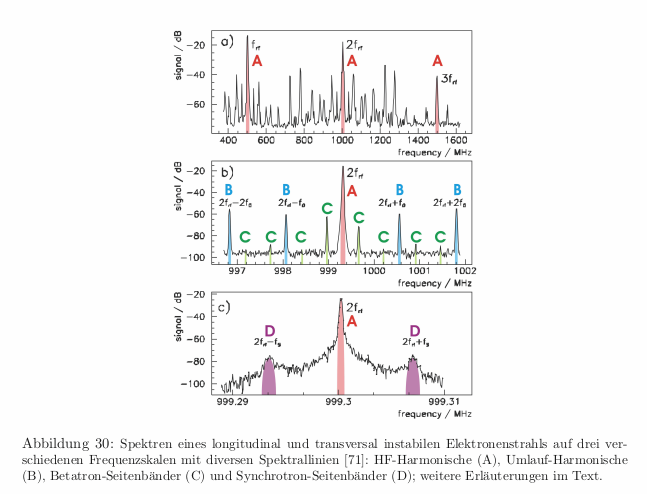
\includegraphics[width=\textwidth]{sprektrum.png}
			\end{figure}
		
		\item[n)]
			Wake-Felder sind Felder, die die Strahlteilchen selber erzeugen.
			Die Strahlteilchen erzeugen in der Vakuumkammer ein elektrisches Feld,
			welches sich auf Grund der endlichen Leitfähigkeit nicht instantan abbauen kann.
			Im Frequenzraum ist die Impedanz das analogon zum ohmschen Wiederstand.
		
		\item[o)]   
			Eine schmalbandige Impedanz als Instabilitätsmechanismus entspricht der Grundmode der HF-Resonatoren. Grundfrequenz dieser wird so eingestellt, das sie
			etwas unterhalb der Umlaufharmoinischen ist.
		
		
		\item[p)]      
			\begin{itemize}
				\item Einteilchen-Modell (Teilchenpaket als ein Makroteilchen): multi bunch- Instabilitäten
				\item Zweiteilchen-Modell: head-teil-Instabilität
				\item kontinuerliche Ladungsverteilung: kopliziertere Moden innerhalb eines Pakets simulieren
			\end{itemize}


	\end{itemize}

\end{document}